\documentclass[10pt]{article}
\usepackage{amsmath}
\usepackage{graphicx}
\usepackage{float}
\usepackage{subfigure}
\usepackage{listings}
\usepackage{booktabs}
\usepackage{xcolor}
\usepackage{longtable}
\usepackage{geometry}
\geometry{b5paper,left=1cm,right=1cm,top=1cm,bottom=2cm}
\usepackage{karnaugh-map}
\usepackage{verbatim}
\usepackage{tikz}
\usepackage{xparse}
\usepackage{tikz-timing}
\usetikzlibrary{automata, positioning, arrows}
\usepackage{textcomp}
\begin{document}

\title{TEA - Tiny Encryption Algorithm}
\maketitle
\tableofcontents



\section{algorithm}

\begin{figure}[H]
\centering
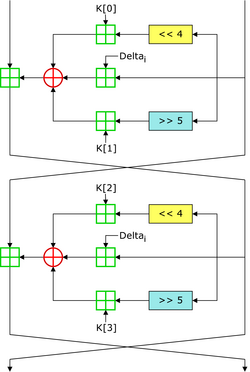
\includegraphics[width=0.4\textwidth]{TEA_InfoBox_Diagram.png}
\caption{TEA one-round (image from wikipedia)}
\label{TEA_InfoBox_Diagram.png}
\end{figure}



\section{design}

\begin{figure}[H]
\centering
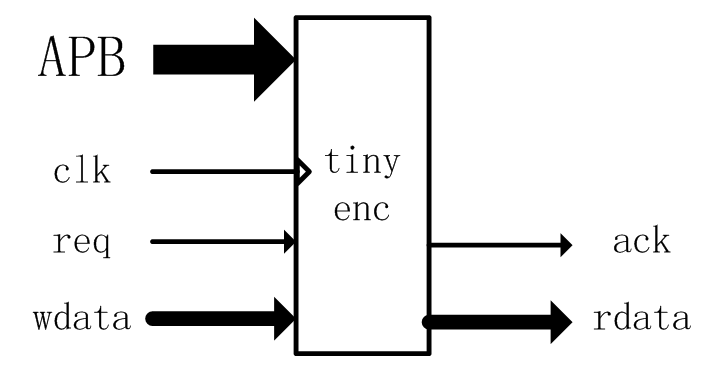
\includegraphics[height=0.2\textwidth]{20250805121912_711x381_scrot.png}
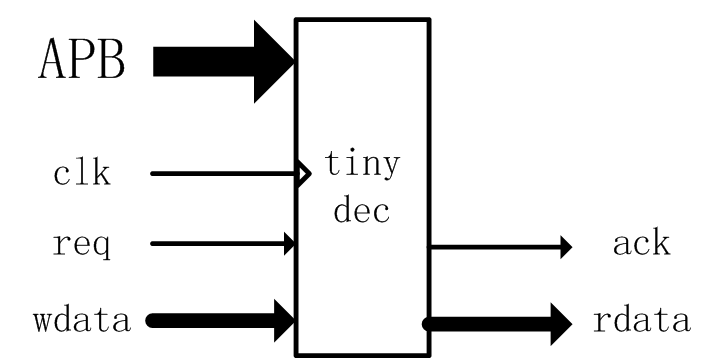
\includegraphics[height=0.2\textwidth]{20250805121919_706x364_scrot.png}
\caption{Design}
\label{20250805121619_706x366_scrot.png}
\end{figure}




\subsection{registers}

\begin{table}[H]
\begin{tabular}[width=\textwidth]{|l|l|l|}
\hline
reg                        &offset	 &description \\
\hline
key10                      &0x0      &key[31:00]  \\
key32                      &0x4      &key[63:32]  \\
delta                      &0x8      &delta       \\
\hline
\end{tabular}
\label{t1}
\caption{registers}
\end{table}

\begin{table}[H]
\begin{tabular}[width=\textwidth]{|l|l|l|l|}
\hline
signal        &offset   &type &description   \\
\hline
key0           &[15:00]    &RW   &key[15:00] \\
key1           &[31:16]    &RW   &key[31:16] \\
\hline
\end{tabular}
\label{t1}
\caption{reg: key10}
\end{table}

\begin{table}[H]
\begin{tabular}[width=\textwidth]{|l|l|l|l|}
\hline
signal        &offset   &type &description   \\
\hline
key2           &[15:00]    &RW   &key[47:32] \\
key3           &[31:16]    &RW   &key[63:48] \\
\hline
\end{tabular}
\label{t1}
\caption{reg: key32}
\end{table}


\begin{table}[H]
\begin{tabular}[width=\textwidth]{|l|l|l|l|}
\hline
signal        &offset   &type &description \\
\hline
delta         &[16:00]   &RW   &delta \\
\hline
\end{tabular}
\label{t1}
\caption{reg: delta}
\end{table}




\end{document}
